\documentclass[12pt,a4paper]{article}

\usepackage{url}
\usepackage{appendix}
\usepackage[british]{babel}
\usepackage{amsmath}
\usepackage{hyperref}
\usepackage{graphicx}
\numberwithin{equation}{section}
\numberwithin{figure}{section}
\numberwithin{table}{section}

\usepackage[round]{natbib}
\bibliographystyle{natbib}
\def\bibsection{\section*{References}}

% Wrap around which gives all figures included the [H] command, or places it "here". This can be tedious to code in Rmarkdown.
\usepackage{float}
\let\origfigure\figure
\let\endorigfigure\endfigure
\renewenvironment{figure}[1][2] {
    \expandafter\origfigure\expandafter[H]
} {
    \endorigfigure
}

\let\origtable\table
\let\endorigtable\endtable
\renewenvironment{table}[1][2] {
    \expandafter\origtable\expandafter[H]
} {
    \endorigtable
}

\def\tightlist{}

\bibpunct[:]{(}{)}{;}{a}{,}{,}

\renewcommand{\baselinestretch}{1.5}

\begin{document}

\begin{titlepage}

\begin{center}
{\Huge \bf Comparing rolling period forecasts of Facebooks' Prophet model to an
ARIMA model: A Diebold-Mariano evaluation of the FTSE/JSE Top40 Index}\\
\today\\
Marvelous Mubenesha ( MBNMAR005)\\
{\tt MBNMAR005@myuct.co.za}
\end{center}

\begin{abstract}
Facebook's data science team open-sourced Prophet, a package that allows
analysts to forecast a wide range of business time series at-scale.
Prophet employs intensive Bayesian modelling in two tiers. Purely
through MAP parameter estimation, and in a quasi-Bayesian form through
an automated forecast evaluation that enables analyst to improve a
forecasting model if it underperforms when compared to other traditional
models. This paper assesses the predictive accuracy of Prophets'
forecasts to those of an ARIMA model that was identified using the
Box-Jenkins methodology. This is achieved through a Diebold-Mariano
evaluation of the rolling period forecast errors of returns on the
FTSE/JSE Top40 Index across daily, weekly and monthly time horizons. The
results of the study suggest that there is insufficient evidence to
conclude that the forecasting models have unequal predictive ability
within the scope of the FTSE/JSE Top40 Index.
\noindent
Keywords: prophet forecasting, arima forecasting, Box-Jenkins methodology,Diebold-Mariano test,multi-step rolling window forecasts, FTSE/JSE Top40 index.
\end{abstract}
\end{titlepage}

\pagenumbering{arabic}

\section{\texorpdfstring{Introduction\label{Introduction}}{Introduction}}\label{introduction}

In business, including that involving the stock market, analysts require
a large number of time series forecasts to inform decision making. The
challenge with existing reliable approaches to forecasting time series
data are that the models require a considerable background in statistics
to build and adapt to prevailing market conditions when needed. Several
authors have recommended automatic forecasting, which refers to
algorithms that can automatically forecast a large number of univariate
time series. However, the forecasts generated by these methods have been
found to be brittle as well as inflexible in allowing for prior
information to be incorporated into the forecasting model (Taylor and
Letham 2017). In February of 2017, Facebook's Core Datascience team open
sourced Prophet, a time series forecasting tool with unique features
that enable ``forecasting-at-scale''. Forecasting-at-scale is a term
coined by the data science team which they define as, ``an approach that
allows a large number of analysts to forecast a large number and variety
of business time series'' (Taylor and Letham 2017). It has the added
advantage of being less `expensive' than other alternatives. In
addition, it is specifically preferable over ARIMA models because of its
non-linearity, flexibility and ability to accomodate varying time
intervals (Taylor and Letham 2017).

The objective of this paper is to compare the rolling period forecasts
generated by Prophet (which uses automated, intensive Bayesian Modelling
to `forecast-at-scale'), to those obtained from an ARIMA model
(constructed through the Box-Jenkins methodology), through a
Diebold-Mariano evaluation of the FTSE/JSE Top40 Index. The study is
particularly useful because analysts from a wide background can reliably
forecast stock price returns automatically, and incorporate their prior
knowledge in the forecasting model, without a wholesome understanding of
the statistical intricacies involved. It is hoped that this could create
opportunities for automated invesment mechanisms.

The paper is organized as follows. A review of literature relating to
stock price forecasting with ARIMA models and other alternative
approaches is introduced in section 2.1 to give the reader background
information on existing research relating to the subject matter.
Thereafter, theory relating to the mathematical formulation and
estimation of an ARIMA and Prophet model is included in sections 2.2 and
2.3 respectively. Subsequently, in section 2.4, the theoretical
motivation and mathematical formulation of the Diebold-Mariano test is
introduced as a means of comparing the predictive accuracy of two
prediction models. Information relating to the data that was used in
this study is contained in section 3, after which, the methodology used
to answer the research question is described in section 4. Section 5,
contains the results obtained when the methodology was executed, whilst
section 6 includes a discussion of the results. The discussion includes
a response to the research question as well as some useful insights from
the results. Furthermore, it highlights some recommendations for further
areas of research based on the findings of the paper. Lastly, the
conclusion in section 7 summarizes the results of the study relative to
the main objective of the paper.

\section{Background}\label{background}

In this section we will briefly review literature that relates to the
comparison of different approaches to forecasting stock returns. This
will include both traditional approaches as well as relatively new
methods such as automatic forecasting, machine learning techniques and
quasi-Bayesian forms which incorporate analysts' prior information. The
theoretical and mathematical formulation of an ARIMA forecasting model
is then briefly introduced. Thereafter, the theoretical framework and
mathematical formulation of Facebooks' Prophet forecasting tool is
discussed. Specific attention is drawn to Prophets distinguising
features to give the reader an understanding of the value that this
forecasting technique can potentially add to stock price prediction. The
background information is concluded with an introduction to the
Diebold-Mariano Evaluation as a suitable framework to formally compare
the predictive accuracy of two forecasting models.

\subsection{Literature}\label{literature}

\subsubsection{Forecasting stock prices using the ARIMA
model}\label{forecasting-stock-prices-using-the-arima-model}

ARIMA models have been widely used as a standard model to forecast
financial data and have been shown to yield forecasting errors that lie
within acceptable bounds (Adebiyi, Adewumi, and Ayo 2014). Adebiyi,
Adewumi, and Ayo (2014) used the Box-Jenkins methodology to build
short-term stock price prediction models for stocks on the New York
Stock Exchange(NYSE) and the Nigerian Stock Exchange(NSE). Their results
showed that the predictive power of the ARIMA model was satisfactory
based on forecast error diagnostics.

ARIMA models rely on the assumption that residuals are
homoskedastic(they have a constant variance) and normally distributed.
However, the residual errors of some financial data display
heteroskedasticity making GARCH models more applicable. This theory is
backed by a study conducted by Mutendadzamera and Mutasa (2014) who
compared the ability of ARIMA and GARCH models to forecast stock prices
on the Zimbabwean Stock Exchange (ZSE). They found that the GARCH model
outperforms the ARIMA model which suggests that incorporating
heteroskedasticity of the residual errors improves the forecasting
ability of the model. This is a case in point for emerging market
stocks. The researchers noted that poor liquidity in the market could be
a cause of the results they observed (Mutendadzamera and Mutasa 2014).

\subsubsection{Forecasting stock prices using alternative methods: The
case of Artificial Neural Networks and Hybrid
Models}\label{forecasting-stock-prices-using-alternative-methods-the-case-of-artificial-neural-networks-and-hybrid-models}

Though the ARIMA model is tractable given that it is simple,
interpretable and yields forecasts that are significantly accurate when
compared to other methods, it has its limitations. The most popular
being its inability to capture non-linear patterns in data, even after
its evolution from the standard form to more adaptable formulations
(Moreno, Pol, and Gracia 2011). Over the past two to three decades with
the evolution of computational power and statistical advancement, other
stock price prediction methods have been proposed, the most prominent
being a machine learning approach called Artificial Neural
Networks(ANNs) (Lin, Yang, and Song 2009). Also popular amongst the new
stock price forecasting approaches are hybrids of existing methods that
incorporate the benefits of different approaches.

An Artificial Neural Networks (ANNs) is a multi-layered perceptron with
nodes that simulate the action of neurons as illustrated in figure 1.\\
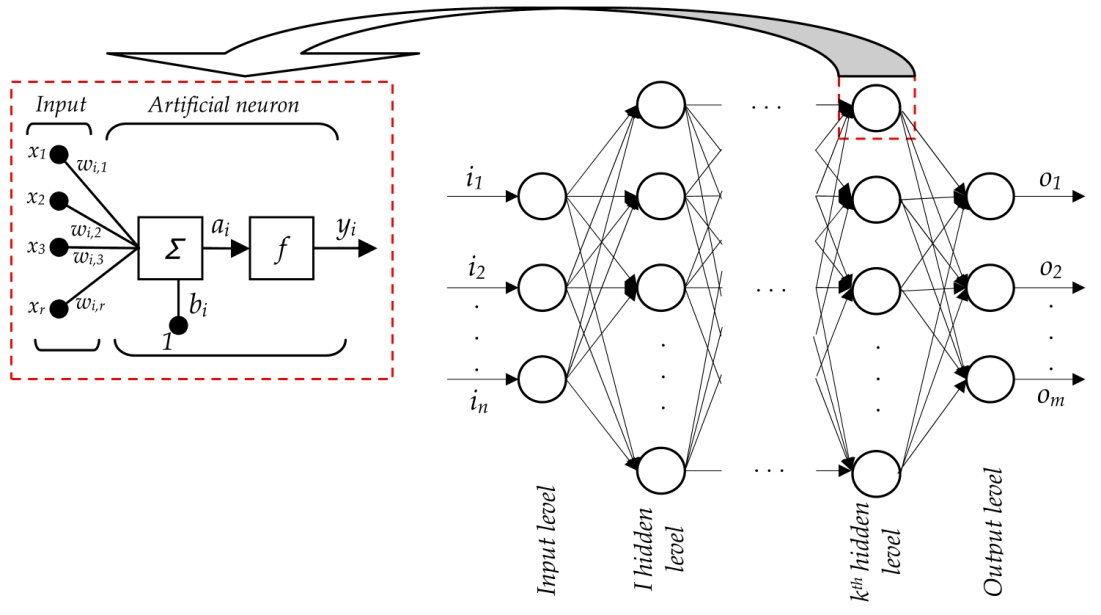
\includegraphics{ANN.png}\\
\emph{Figure 1 : Illustration of an Artificial neural network} (Tanikic
and Despotovic 2012)\\
Formally, an ANN consists of a sorted triple \((K, A, \omega)\). \(K\)
is a set representing the multiple levels of the network i.e.~input,
hidden and output levels. A is a set of pairs that represents the index
for the estimated parameter at the \(i^{th}\) node of the \(k^{th}\)
level in the network. This is illustrated by the curved down arrow in
Figure 1 which points to an enlarged segment of the \(i^{th}\) node in
the \(k^{th}\) level i.e. \(a_{i,k} \in A\). Lastly, \(\omega\)
represents a function that defines the weights (\(\omega_{i,r}\)) of
connections between nodes that interact across adjacent levels (Kriesel
2007). Artificial Neural networks apply iterated optimization of model
parameters across the network in the form of weights conditional on
observed values to learn (Segaran 2007). Several studies have compared
ARIMA model forecasts to ANN and their conclusions are contradictory.

Researchers have found that the performance of either method depends on
the nature of the data and forecasting problem (Kihoro, Otieno, and
Wafula 2004). Stock price data is proposed to be nonlinear which
suggests that nonlinear approaches have the potential to produce better
forecasts than linear models. Furthermore, ANNs make no assumptions
about the distribution of the errors as compared to the linear ARIMA
model (Adebiyi, Adewumi, and Ayo 2014). Adebiyi, Adewumi, and Ayo (2014)
compared NYSE stock index forecasts of an ARIMA model to those of an ANN
and found that the forecasting accuracy of the ANN model was superior to
that of the ARIMA model. It is evident that ANN are preferred to ARIMA
models as a model free, nonlinear alternative. However, the model
construction of an ANN requires trial and error to initialize parameter
estimates and these parameters are not easily interpretable by analysts
(Moreno, Pol, and Gracia 2011). Researchers have found different ways to
guide analysts in this respect. In 1996, Wang and Leu (1996) proposed an
ARIMA-based ANN to forecast the medium-term price of the Taiwan Stock
Exchange Weighted Stock Index (TSEWSI). They used the Box-Jenkins
methodology to difference the series and then trained the data on a
neural network with initialisations that were guided by their
observations of the ARIMA model. Their hybrid model yielded forecasts
that were comparably superior to the individual models used in isolation
based on an analysis of the out-of-sample residual error diagnostics.
Wang and Leu (1996) therefore concluded that the ARIMA-based Neural
Network outperformed a Neural Network trained using raw stock price data
(Wang and Leu 1996). Zhang and Wu (2009) used a combination of the
backpropagation algorithm from Neural Networks with Improved Bacterial
Chemotaxis Optimization (IBCO) to build a model that forecasts the S\&P
500 stock index by minimizing the mean square error. Model forecasts
were evaluated through simulation experiments and the results led to the
conclusion that the hybrid model produced superior forecasts (Zhang and
Wu 2009). This study further highlighted the potential that nonlinear
approaches have in forecasting stock prices. An issue that arises with
such methods is the complexity of the proposed models which limits the
flexibility of unseasoned analysts to adjust model parameters as a way
of improving forecasting accuracy. As we will see, Prophet elegantly
deals with this issue in the form of a nonlinear, Generalized Additive
Model (GAM).

\subsubsection{Quasi-Bayesian forecasting methods that incorporate an
analysts'
knowledge}\label{quasi-bayesian-forecasting-methods-that-incorporate-an-analysts-knowledge}

The stock price forecasting approaches considered so far purely apply
technical data analysis methods to generate stock price forecasting
models. However, studies that have compared pure technical approaches to
those that incorporate an analysts knowledge in a quasi-Bayesian form
have been shown to be superior at predicting market prices (Givoly and
Lakonishok 1984 \& Guerard (1989)). The first instance of combining
time-series model forecasts and an analysts forecasts to obtain superior
forecasts of a stocks annual earnings can be dated to 1989. Guerard
(1989) used an additive model to combine consensus security analyst
forecasts from the S\&P Annual Earnings forecaster and annual earnings
forecasts generated by an ARIMA model with a nonzero mean. The combined
model that was estimated using ordinary least squares reduced the mean
square error of the time series and analysts forecasts from 1.28 and
1.27, respectively to 1.04. These results suggest that analysts can
reduce forecasting errors by combining technical methods with expertise
developed through market knowledge (Guerard 1989). Zahedi and Rounaghi
(2015) applied the same overarching principle when they used principle
component analysis to determine an appropriate input variable which they
then used to train an ANN in an attempt to predict stock prices on the
Tehran Stock Exchange. Their model yielded reduced forecasting errors
and performed better than the pure ANN. These results further reiterate
the potential of incorporating an analysts knowledge to improve stock
price forecasts, in both linear and nonlinear models.

\subsection{ARIMA model formulation}\label{arima-model-formulation}

The ARIMA model is a generalisation of Autoregressive Moving Average
(ARMA) models which combine autoregression and moving average features
(Box and Jenkins 1970). In the context of returns, the ARIMA formulation
for the return at time index \(t\), \(r_t\), is given by,
\[  r_t = \phi_1 r_{t-1} + \phi_2 r_{t-2} + ...+ \phi_p r_{t-p} + \epsilon_t +
        \psi_1 \epsilon_{t-1} + \psi_2 \epsilon_{t-2} + ... +\psi_q \epsilon_{t-q} \]where:\\
\(\bullet\) \(\phi_i\) and \(\psi_j\) are the parameters to be
estimated\\
\(\bullet\) \(r_{t-k}\) is the \(k^{th}\) lagged return\\
\(\bullet\) \(\epsilon_t\) is the error term at time \(t\) which is
assumed to be white noise\\
\(\bullet\) \(\epsilon_{t-k}\) is the \(k^{th}\) lagged error\\
\(\bullet\) \(p\) is the order of the autoregressive component
(dependence on history of \(r_t\)) and\\
\(\bullet\) \(q\) is the order of the moving average component
(dependence on history of \(\epsilon_t\)).

The ARIMA model will be used as a standard forecasting method which
Prophet will be compared against. Model building and parameter
estimation will follow the approach outlined by Box and Jenkins (1970)
and is further discussed in the methodology

\subsection{Prophet model formulation and
estimation}\label{prophet-model-formulation-and-estimation}

The challenge with many forecasting methods such as the Box-Jenkins
methodology and machine learning approaches discussed in the literature
review are that they usually require a sufficient statistical background
to construct and modify if necessary. Furthermore, some of these
approaches tend to be inflexible with respect to incorporating prior
information. In some instances, such as with ANN, incorporating prior
information can be partially achieved through initializing parameter
estimates. However, an analyst with limited statistical training can
have difficulty interpreting and thus modifying initial parameter
estimates (Taylor and Letham 2017).\\
Prophet is an \textbf{automatic forecasting} tool that uses a Bayesian
Generalized Additive model to generate time series forecasts. This is in
comparison to conventional methods such as the linear stochastic
dependence that exists in ARIMA models. Prophet combines a configurable
model that includes an automated evaluation of forecasts with the
interaction of an analyst in the loop (Taylor and Letham 2017). The
model is configurable which allows an analyst to incorporate their
knowledge of the behaviour of the series into the model building process
through easily interpretable initial parameters that can be modified and
interactive feedback when forecasts under-perform (Taylor and Letham
2017).

Through this mechanism, a large number of forecasts can be reliably
generated \textbf{automatically} with the flexibility of enabling an
analyst to modify the model in-the-loop during model specification. The
automated forecasting procedure with an analyst-in-the-loop is
illustrated in Figure 2.

The first step of the forecasting procedure begins with the analyst
simply specifying a general model (i.e.~modelling). Prophet then goes
into the automated process of estimating model parameters and performing
forecast evaluation. Automated forecast evaluation is undertaken by
constructing baseline forecasts using methods such as the sample mean,
ARIMA, exponential smoothing and naive estimates (e.g.~last value or
seasonal last value). Thereafter, simulated historical forecasting (SHF)
errors are evaluated by comparing forecasts of the baseline methods and
prophet to the observed historical values. SHF errors are forecast
errors generated by random points in the history of a time series model.
Prophets SHF errors that are relatively large compared to the baseline
methods are then surfaced with visual illustrations of the results. The
process then transitions from surface problems to the top left of the
cycle in Figure 2 labelled analyst-in-the-loop. Here, the analyst can
then visually inspect forecasts to identify issues and modify features
of the Prophet model before it is re-estimated in the modelling stage.
The loop is repeated until forecast evaluation surfaces no problems
(Taylor and Letham 2017).

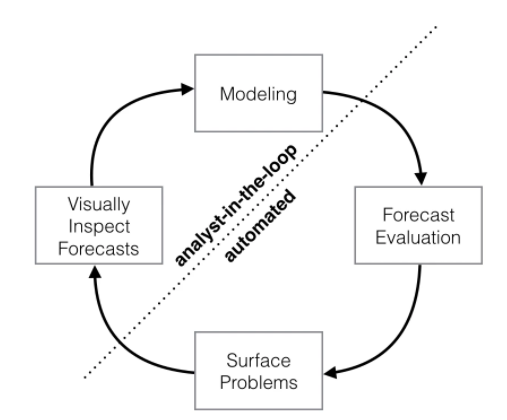
\includegraphics[width=0.80000\textwidth]{analyst in the loop.png}\\
\emph{Figure 2: Illustration of Prophets' automated forecasting
procedure with an analyst in the loop} (Taylor and Letham 2017)

The interpretability of Prophets' model parameters stems from the
mathematical formulation of the generalised additive model. The
formulation posits that the series is generated by an additive,
parametric function of time \(r(t)\), defined by,
\[ r(t) = g(t) + s(t) +  h(t) + \epsilon_t.\] The additive components
include growth, seasonality and a component that adjusts for holidays as
well as once-off events e.g.~anticipated market shocks in the instance
of financial time series.

Firstly, the growth component, \(g(t)\), is modelled using a generalized
form of the logistic population growth model and is of the form;\\
\[g(t) = \frac{C(t)}{1+exp(-(k+\boldsymbol{a}(t)^T \delta(t-(b+\boldsymbol{a}(t)^T \gamma)))}\]\\
where:\\
\(\bullet\) \(C(t)\) represents the carrying capacity of the growth
component and can be modelled using a polynomial function of time, the
simplest being a constant or linear model.\\
\(\bullet\) \((k+\boldsymbol{a}(t)^T\delta)\) is the growth rate factor
with the \(\boldsymbol{a}(t)^T\delta\) term enabling the forecaster to
choose where the growth rate changes( i.e change points) and\\
\(\bullet\) \((b+\boldsymbol{a}(t)^T \gamma)\) is the adjusted offset
parameter.\\
The growth component of the model has two useful features that allow the
carrying capacity and growth rate of the model to vary with time. This
enables an analyst to manually define when and how the growth rate
changes at different change points (Taylor and Letham 2017). This
feature is particularly useful for forecasting stock price data since
analysts are able to incorporate market movements that lead to the
growth rate either decreasing, increasing or becoming constant.

Secondly, the seasonality component, \(s(t)\) with periodicity \(P\) is
given by, \[s(t) = \sum_{n = -N}^{N}c_n \exp(j\frac{2\pi nt}{P})\]

Yearly and weekly seasonality is modelled using the standard Fourier
series. Analysts can thus use prior knowledge to account for the effects
of periodicities they have observed seasonally.

Lastly, \(h(t)\) is the holiday and events component, a feature that
ARIMA models are not adapted to. The holiday component enables analysts
to incorporate shocks and once-off events that do not follow a periodic
pattern but may have an effect on the price of a stock. Holidays and
events are modelled using,

\[ h(t) = \sum_{j = 1}^{L}\kappa_j \boldsymbol{1}(t \in D_j) \label{eqn5}
\] Where, \(\kappa\) is a normally distributed scaling factor and
\(D_j\) is a set of past and future dates where holidays or events
occur.

Prophet translates model parameter estimation into a curve-fitting
exercise by employing Maximum Apriori Posterior (MAP) estimation, a
Bayesian approach to estimating optimal parameter values for the
forecasting model. MAP estimation finds the maximum posterior estimates
for the parameters by using the likelihood function and an apriori
distribution to evaluate a posterior distribution which is then
optimized to return point estimates of the parameters (Taylor and Letham
2017).

\subsection{Diebold-Mariano
evaluation}\label{diebold-mariano-evaluation}

As is evident from sections 2.2 and 2.3, the modelling approach and
assumptions of Prophet differ to those of an ARIMA model. Since the two
methods differ, the Diebold-Mariano evaluation is preferred as a means
of formally comparing the forecasting accuracy of the two models
statistically. The Diebold-Mariano evaluation is a \textbf{model free}
hypothesis test for the equal predictive accuracy of two forecasting
methods, referred to as model 1 and model 2. It is applicable to a wide
range of situations from forecast residuals that are non-Gaussian,
asymmetric loss functions, serially correlated errors and multi-period
forecasts (Mariano 2000). The Diebold-Mariano test (DM test) operates by
evaluating the forecast errors for both model 1 and model 2 (i.e
\(e_{t_1}\) and \(e_{t_2}\)) at a loss function \(g(\bullet)\). The loss
function can be choosen flexibly as long as it is zero when the error is
zero, is strictly positive for all values on the real line and, it
increases with an increase in the absolute value of the error size. The
loss differential between two forecasts at time \(t\) is then defined
by, \[ d_t =  g(e_{t1}) - g(e_{t2})\] for \(t = (1, 2, ..., M)\) where
\(M\) is the total number of forecasts that have been generated from
each model. We then test whether, \[ \mu = E[d_t] = 0 \] by conducting
the following hypothesis test;\\
Null hypothesis: \[ E[d_t] = 0  \,\,\,\, \forall t\]\\
Alternative hypothesis: \[ E[d_t] \neq 0 \]\\
Test statistic:
\[DM_{stat} = \frac{\sqrt M (\bar{d} - \mu)}{\sqrt{\hat{\gamma_d(0)}}} \]

\(\bar{d}\) is the sample mean of the \(M\) loss differentials and
\(\frac{\hat{\gamma_d(0)}}{M}\) is the asymptotic variance of
(\(\bar{d} - \mu\)) with \(\hat{\gamma_d(k)}\) representing the
autocovariance of the loss differential series at lag \(k=0\).
Asymptotically, the \(DM_{stat}\) has a standard normal distribution if
the loss differential series is short memory and covariance stationary
(Mariano 2000).\\
There are two caveats to using the DM Test for the purposes of this
paper. Firstly, the choice of the loss function depends on whether the
forecast errors can be assumed to be symmetric or asymmetric. When the
forecast errors are symmetric, a linear or quadratic loss function can
be used to evaluate the loss differential. For forecast errors that are
asymmetric, a loss fuction that satisfies the conditions outlined in the
first part of this section can be used. Secondly, literature does not
clearly stipulate the sample size range that is sufficient for the
asymptotic distribution assumption to hold. In light of this, relatively
large sample sizes were used in this study and the DM test results are
applied conservatively.

\section{Data}\label{data}

The data set used throughout this paper comprises of the daily closing
prices of the FTSE/JSE Top40 price index for the five year period from
31/07/2012 to 31/07/2017. This equates to a total of 1305 trading days
excluding weekends and holidays. This period was chosen for its recency
and to avoid exposing the results to the noise associated with the high
volatility experienced in the stock market during the 2008 financial
crisis. The aim is to compare the predictive accuracy of the two models
under standard market conditions before other confounding factors can be
closely analysed. Figure 3 shows the actual realisations of the price
index data which was sourced from Datastream.

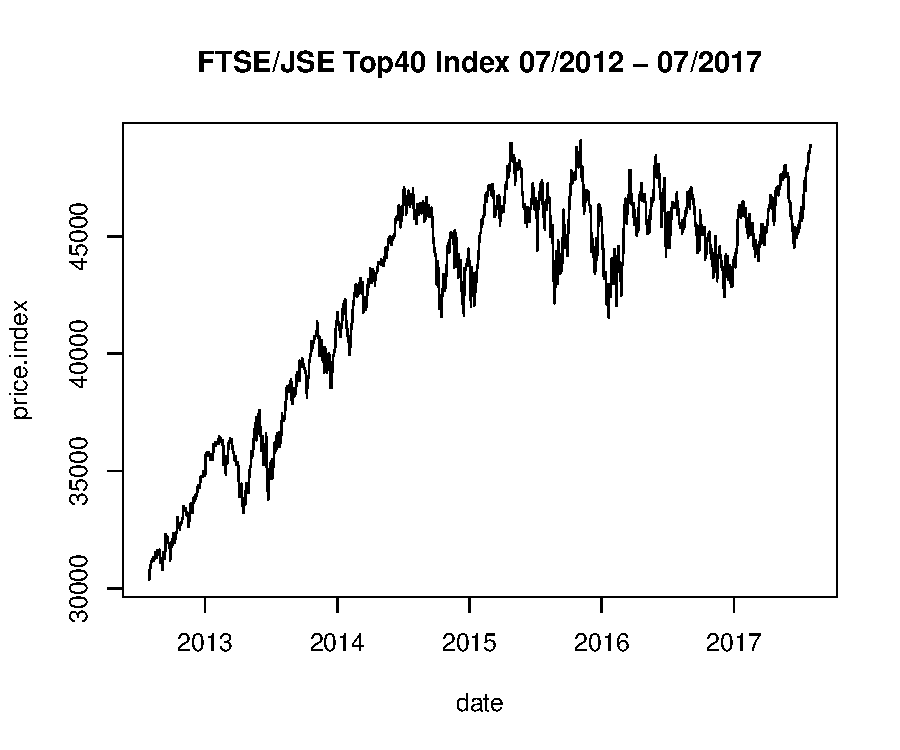
\includegraphics{Draft_Paper_files/figure-latex/unnamed-chunk-1-1.pdf}
\emph{Figure 3: Realisation of the FTSE/JSE Top40 Price Index over the
period of study}

The price index was transformed to log returns as a means of avoiding
spurious regression issues which can be caused by the existence of unit
roots in stock price data.

In this paper, the \textbf{log return} (which will be used
interchangeably with \textbf{return}), over the period \([t,t+1]\) is
denoted by \(r_t\), and was calculated by evaluating;\\
\[
r_t = log(\frac{P_{t+1}}{P_t})  \label{eq1}
\]\\
Where \(P_t\) and \(P_{t+1}\) represent the price of the index at time
\(t\) and \(t+1\) respectively.

\section{Methodology}\label{methodology}

Preliminary data processing was done to clean and transform the data
before formally testing for outliers. The data was then split into
in-sample and out-of-sample periods. As was mentioned in section 2.4,
literature does not clearly stipulate what sample size is sufficient for
the asymptotic distribution assumption to hold. In response to this,
20\% of the available data was used as the out-of-sample period. The
in-sample period comprises of 1044 trading days between 30 July 2012 to
the 31 July 2016 whereas the out-of-sample period comprises of the
trading days between 1 August 2016 and 31 July 2017.

The in-sample data was used to identify the ARIMA forecasting model
using the method outlined by Box and Jenkins (1970) for building and
estimating an ARIMA model.\\
Thereafter, one-step rolling forecasts with re-estimation as outlined by
Hyndman (2014) were evaluated for an automated Prophet model and the
ARIMA model that was identified using the Box-Jenkins methodology. This
procedure was then repeated for a 5-step and 20-step forecast horizon in
order to determine whether the performance of the models vary when
estimating daily,weekly or monthly stock returns.

The forecasts generated above were then used to calculate \textbf{h-step
rolling forecast errors} for both the ARIMA and Prophet model. For each
time point \(t\) in the out-of-sample period, the rolling forecast error
is given by,

\[ \hat{e_t} = r_t - \hat{r_t},\] where \(r_t\) is the actual return and
\(\hat{r_t}\) is the rolling forecast at time \(t\).

Summary statistics of the errors where used to compare the performance
of the forecasting models before a formal statistical test was performed
using the DM test with a linear and quadratic loss function. Using
either a linear or quadratic loss function implicitly assumes that the
forecast errors are symmetric (Mariano 2000). This assumption is
reasonable given the apparent symmetry in the distribution of forecast
errors as is evident from the boxplots in Figure 5, section 5.2.

\section{Results}\label{results}

\subsection{Box-Jenkins methodology: ARIMA model identification and
selection}\label{box-jenkins-methodology-arima-model-identification-and-selection}

The methodology as outlined in Box and Jenkins (1970) was applied to the
data through the following procedure. The stationarity of the time
series was tested formally by performing an Augmented Dickey-Fuller test
on the in-sample log returns data. The test yielded a p-value less than
1\% which implies that we reject the null hypothesis which states that
the in-sample returns series non-stationary.

The autocorrelation(ACF) and partial autocorrelation(PACF) functions in
Figure 4 were used to identify candidate \emph{ARIMA(p,d,q)} models to
fit to the in-sample data. The results suggest that the second lag of
both functions might be significantly different from zero.

\begin{center}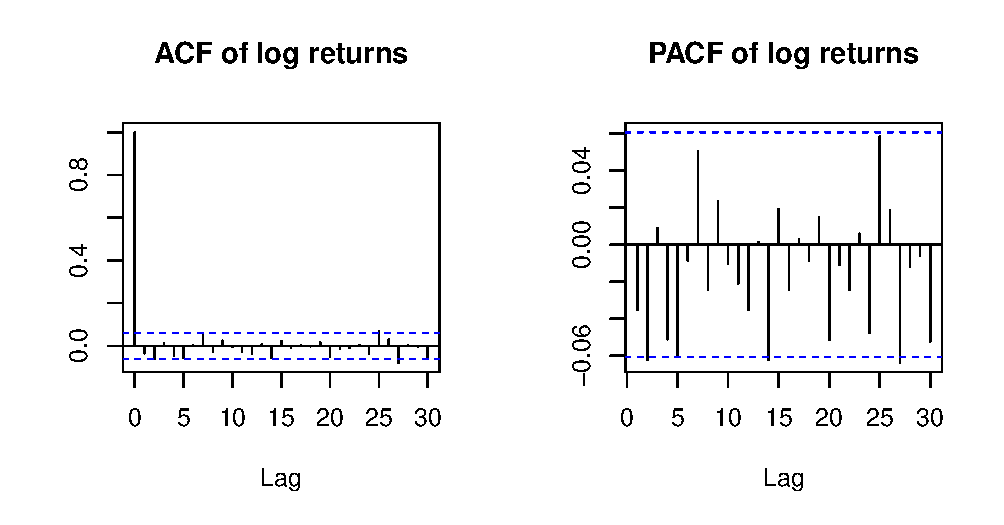
\includegraphics{Draft_Paper_files/figure-latex/acf_and_pacf_plot-1} \end{center}

\emph{Figure 4 : ACF and PACF plots for in-sample data}

The candidate models that were fit to the in-sample data are shown in
Table 1 with their respective AIC values. The \(ARIMA(2,0,2)\) model had
the lowest AIC and was thus selected as the ARIMA forecasting model.

\emph{Table 1: AIC for candidate ARIMA models}

\begin{table}[H]
\centering
\begin{tabular}{ll}
  \hline
ARIMA(p,d,q) model & AIC \\ 
  \hline
(0,0,0) & -8804 \\ 
  (2,0,0) & -8808 \\ 
  (0,0,2) & -8808 \\ 
  (2,0,2) & -8817 \\ 
   \hline
\end{tabular}
\end{table}

\subsection{Forecast error evaluation}\label{forecast-error-evaluation}

The results of model estimation and forecast evaluation using the
rolling window for h-step forecasts yielded forecasts errors with
roughly equal distributions. This is visible from the boxplot in Figure
5. The presence of outliers seems consistent across the different models
\textbf{and} forecasting horizons. Furthermore, variations in accuracy
across different forecasting horizons \emph{for each} model is not
observable in Figure 5. The mean error and spread of both models across
different time horizons appears to be constant.

\begin{figure}

\begin{center}\includegraphics{Draft_Paper_files/figure-latex/box_plot-1} \end{center}
\end{figure}

\emph{Figure 5: Boxplot illustrating distribution of rolling forecast
errors for different time horizons, h}

\subsubsection{Forecast Error
Statistics}\label{forecast-error-statistics}

Table 2 summarizes the forecast error statistics for both the ARIMA and
Prophet model across the three different time horizons.\\
Across all forecast horizons, the ARIMA model appears to be
overestimating returns. This is evident from the negative mean error(ME)
across \(h = (1,5,20)\). On the contrary, the Prophet model
underestimates the forecasts for one-step and five-step ahead
forecasting horizons. It then overstimates returns when forecasting
twenty-steps ahead. The ME results shown in Table 2 fail to clearly
illustrate which model performs better. Furthermore, the ME values are
relatively small when compared against other error statistics.

\begin{table}[H]
\centering
\caption{Forecast error diagnostic statistics over different forecasting horizons} 
\begin{tabular}{lllll}
  \hline
Forecast Horizon, h & Forecast Model &  ME  & RMSE & MAE \\ 
  \hline
1 & ARIMA & -0.0004110 & 0.0103 & 0.007718 \\ 
    & Prophet & 0.0000176 & 0.0104 & 0.007749 \\ 
  5 & ARIMA & -0.0003635 & 0.0103 & 0.007692 \\ 
    & Prophet & 0.004445 & 0.0103 & 0.007709 \\ 
  20 & ARIMA & -0.0001769 & 0.0102 & 0.007649 \\ 
    & Prophet & -0.0000406 & 0.0102 & 0.007660 \\ 
   \hline
\end{tabular}
\end{table}

The Root Mean Square Error (RMSE) across different forecast horizons and
across both models are considerably close to each other in value
relative to the other error statistics. The same observation can be made
for the Mean Absolute Errors (MAE). These results suggest that the
models possibly have the same forecasting accuracy.

\subsubsection{Diebold-Mariano
Evaluation}\label{diebold-mariano-evaluation-1}

The observations made from Table 2 in section 5.2.1 suggest that the
ARIMA and Prophet models have equal predictive accuracy. These
assertions can be formally quantified through a Diebold-Mariano(DM) test
which evaluates whether the models have equal predictive accuracy
against the alternative hypothesis that one model has superior accuracy
over the other. Table 3 reports the results obtained when the rolling
forecast errors were formally compared against each other over different
time horizons.

\begin{table}[H]
\centering
\caption{Results of the Diebold-Mariano Hypothesis Test for different loss functions} 
\begin{tabular}{lll}
  \hline
Forecast Horizon, h & Loss Function & P Value \\ 
  \hline
1 & Linear & 0.553 \\ 
    & Quadratic & 0.128 \\ 
  5 & Linear & 0.691 \\ 
    & Quadratic & 0.334 \\ 
  20 & Linear & 0.660 \\ 
    & Quadratic & 0.296 \\ 
   \hline
\end{tabular}
\end{table}

The p-value across all the time horizons for either linear and quadratic
loss functions suggest that we would fail to reject the null hypothesis.
This implies that the predictive accuracy of the models could be equal.
These results formally validate the observations made obtained in
section 5.2.1.

\section{Discussion of results}\label{discussion-of-results}

The results of the study show that there is no significant evidence to
conclude that Prophet generates superior forecasts for returns on the
FTSE/JSE Top40 Index when compared against those of an ARIMA model when
the Diebold-Mariano Test is used as a method of evaluation. These
results are consistent for daily, weekly and monthly forecasting
horizons.\\
Nevertheless, the study has flagged the possibility that, on average,
the ARIMA model tends to overestimate forecasted returns on the index
for the forecast horizons under consideration. This is contrary to
Prophet, that, on average, underestimates forecasted returns over daily
and weekly time horizons. This information could be useful for an
analyst engaged in short-term strategies since the choice of the
forecasting model can reflect a particular sentiment or risk appetite.
For example, if the analyst feels like prevailing returns are
underpriced by the market, they might choose to use an ARIMA model,
whereas an opposite sentiment could warrant the use of Prophet.\\
Furthermore, it is worth noting that the merits of Prophet may have not
been fully exposed in this study due to the use of transformed data and
the choice of a forecasting horizon that excluded periods of high
volatility. Nonetheless, it is reassuring that the model has performed
as well as the ARIMA model. This observation could create room for the
application of Prophet in circumstances where flexibility in the model
formulation is desireable.

\section{Conclusion}\label{conclusion}

The challenge of building models that generate superior stock return
forecasts has led to widespread research in the field of quantitative
analysis for decades, but the ARIMA model remains the standard against
which to compare new innovations. This is because of its relative
simplicity and ability to evolve into more complex applications e.g in
the hybrid models considered in the literature review.\\
Prophet has reduced the problem of estimating a time series model to a
curve fittig exercise by defining an additive, parametric function of
time. The functions' parameters are then estimated using Bayesian
estimation methods after which the tool automatically executes forecast
evaluation to optimize its predictive ability.\\
The results of this study suggest that, using a Diebold-Mariano
evaluation, the ARIMA and Prophet forecasting models do not have a
significant difference in predictive accuracy across time horizons of up
to a month. The implications of this are that analysts can then choose
which model to use based on their needs without significantly
compromising forecast accuracy.\\
This study was confined to the analysis of predictive performance during
general market conditions. Further research could explore the predictive
ability of the models during different market conditions. For example,
performance can be compared during bull and bear market conditions or
during periods of high volatility. Additionally, further research can
assess whether prophet would perform better on raw data that has not
been transformed, since the model is built with growth and seasonality
components. This use of which could lead to Prophet models that generate
superior forecasts when compared against alternatives.

\section*{References}\label{references}
\addcontentsline{toc}{section}{References}

\hypertarget{refs}{}
\hypertarget{ref-adebiyi2014comparison}{}
Adebiyi, Ayodele Ariyo, Aderemi Oluyinka Adewumi, and Charles Korede
Ayo. 2014. ``Comparison of Arima and Artificial Neural Networks Models
for Stock Price Prediction.'' \emph{Journal of Applied Mathematics}
2014. Hindawi Publishing Corporation.

\hypertarget{ref-box1970time}{}
Box, George Edward P, and Gwilym M Jenkins. 1970. ``Time Series
Analysis: Forecasting and Control, 1976.'' \emph{ISBN: 0-8162-1104-3}.

\hypertarget{ref-givoly1984quality}{}
Givoly, Dan, and Josef Lakonishok. 1984. ``The Quality of Analysts'
Forecasts of Earnings.'' \emph{Financial Analysts Journal}. JSTOR,
40--47.

\hypertarget{ref-guerard1989combining}{}
Guerard, John B. 1989. ``Combining Time-Series Model Forecasts and
Analysts' Forecasts for Superior Forecasts of Annual Earnings.''
\emph{Financial Analysts Journal}. JSTOR, 69--71.

\hypertarget{ref-RJHyndman2014}{}
Hyndman, Robert J. 2014. ``Variations on Rolling Forecasts.''
\url{https://robjhyndman.com/hyndsight/rolling-forecasts/}.

\hypertarget{ref-kihoro2004seasonal}{}
Kihoro, J, R Otieno, and C Wafula. 2004. ``Seasonal Time Series
Forecasting: A Comparative Study of Arima and Ann Models.'' \emph{AJST}
5 (2).

\hypertarget{ref-kriesel2007brief}{}
Kriesel, David. 2007. ``A Brief Introduction on Neural Networks.''
Citeseer.

\hypertarget{ref-lin2009short}{}
Lin, Xiaowei, Zehong Yang, and Yixu Song. 2009. ``Short-Term Stock Price
Prediction Based on Echo State Networks.'' \emph{Expert Systems with
Applications} 36 (3). Elsevier: 7313--7.

\hypertarget{ref-Mariano2000}{}
Mariano, Robert S. 2000. ``Testing Forecast Accuracy.'' University of
Pennsylvania; Course Notes.

\hypertarget{ref-moreno2011artificial}{}
Moreno, Juan José Montaño, Alfonso Palmer Pol, and Pilar Muñoz Gracia.
2011. ``Artificial Neural Networks Applied to Forecasting Time Series.''
\emph{Psicothema} 23 (2): 322--29.

\hypertarget{ref-Muten2014}{}
Mutendadzamera, S, and Farikayi K Mutasa. 2014. ``Forecasting Stock
Prices on the Zimbabwe Stock Exchange (Zse) Using Arima and Arch/Garch
Models.'' \emph{International Journal of Management Sciences} 3 (6):
419--32.

\hypertarget{ref-segaran2007programming}{}
Segaran, Toby. 2007. \emph{Programming Collective Intelligence: Building
Smart Web 2.0 Applications}. `` O'Reilly Media, Inc.''

\hypertarget{ref-tanikic2012artificial}{}
Tanikic, Dejan, and Vladimir Despotovic. 2012. ``Artificial Intelligence
Techniques for Modelling of Temperature in the Metal Cutting Process.''
In \emph{Metallurgy-Advances in Materials and Processes}. InTech.

\hypertarget{ref-taylor2017forecasting}{}
Taylor, Sean J, and Benjamin Letham. 2017. ``Forecasting at Scale.''

\hypertarget{ref-wang1996stock}{}
Wang, Jung-Hua, and Jia-Yann Leu. 1996. ``Stock Market Trend Prediction
Using Arima-Based Neural Networks.'' In \emph{Neural Networks, 1996.,
Ieee International Conference on}, 4:2160--5. IEEE.

\hypertarget{ref-zahedi2015application}{}
Zahedi, Javad, and Mohammad Mahdi Rounaghi. 2015. ``Application of
Artificial Neural Network Models and Principal Component Analysis Method
in Predicting Stock Prices on Tehran Stock Exchange.'' \emph{Physica A:
Statistical Mechanics and Its Applications} 438. Elsevier: 178--87.

\hypertarget{ref-zhang2009stock}{}
Zhang, Yudong, and Lenan Wu. 2009. ``Stock Market Prediction of S\&P 500
via Combination of Improved Bco Approach and Bp Neural Network.''
\emph{Expert Systems with Applications} 36 (5). Elsevier: 8849--54.

\newpage
\renewcommand{\baselinestretch}{1}
\nocite{*}
\bibliography{}

\end{document}
